{\sl This fieldstone was developed in collaboration with Lukas van de Wiel}.

The domain is an annulus with inner radius $R_1$ and outer radius $R_2$. It is filled with a 
single elastic material characterised by a Young's modulus $E$ and a Poisson ratio $\nu$, a
density $\rho_0$. The gravity ${\bm g}=-g_0 {\bm e}_r$ is pointing towards the center of the domain.

The problem at hand is axisymmetric so that the tangential component of the displacement
vector $v_\theta$ is assumed to be zero as well as all terms containing $\partial_\theta$.
The components of the strain tensor are 
\begin{eqnarray}
\varepsilon_{rr} &=& \frac{\partial v_r}{\partial r} \\
\varepsilon_{\theta\theta} &=& \frac{v_r}{r} + \frac{1}{r} \frac{\partial v_\theta}{\partial \theta}
= \frac{v_r}{r} 
 \\
\varepsilon_{r\theta} &=& \frac{1}{2} \left(   \frac{\partial v_\theta}{\partial r} - \frac{v_\theta}{r} 
+\frac{1}{r} \frac{\partial v_r}{\partial \theta}  \right) =0
\end{eqnarray}
so that the tensor simply is
\begin{equation}
{\bm \varepsilon} =
\left(
\begin{array}{cc}
\varepsilon_{rr} & \varepsilon_{r\theta} \\ 
\varepsilon_{r\theta} & \varepsilon_{\theta\theta} 
\end{array}
\right)
=
\left(
\begin{array}{cc}
\frac{\partial v_r}{\partial r} & 0 \\
0 &  \frac{v_r}{r} 
\end{array}
\right)
\end{equation}
The pressure is
\begin{equation}
p=-\lambda {\bm \nabla}\cdot {\bm v}
= -\lambda \left( \frac{1}{r} \frac{\partial (r v_r)}{\partial r} \right)
\end{equation}
and finally the stress tensor:
\begin{equation}
{\bm \sigma} 
= - p {\bm 1} + 2\mu {\bm \varepsilon}
=  
\left(
\begin{array}{cc}
\lambda \frac{1}{r} \frac{\partial (r v_r)}{\partial r} + 2\mu\frac{\partial v_r}{\partial r} & 0 \\
0 & \lambda \frac{1}{r} \frac{\partial (r v_r)}{\partial r}  +  2 \mu\frac{v_r}{r} 
\end{array}
\right)
\end{equation}
The divergence of the stress tensor is given by \cite{scto01}:
\begin{equation}
{\bm \nabla}\cdot {\bm \sigma} 
=
\left(
\begin{array}{c}
\frac{\partial \sigma_{rr}}{\partial r} + \frac{\sigma_{rr}-\sigma_{\theta\theta}}{r} + \frac{1}{r} \frac{\partial \sigma_{\theta r}}{\partial \theta} \\ \\
\frac{\partial \sigma_{r \theta}}{\partial r} + \frac{1}{r} \frac{\sigma_{\theta\theta}}{\partial \theta}
+\frac{\sigma_{r\theta} + \sigma_{\theta r}}{r}
\end{array}
\right)
\end{equation}
Given the diagonal nature of the stress tensor this simplifies to (also remember that $\partial_\theta =0$):
\begin{equation}
{\bm \nabla}\cdot {\bm \sigma} 
=
\left(
\begin{array}{c}
\frac{\partial \sigma_{rr}}{\partial r} + \frac{\sigma_{rr}-\sigma_{\theta\theta}}{r} \\ \\
0
\end{array}
\right)
\end{equation}
Focusing on the $r$-component of the stress divergence:
\begin{eqnarray}
({\bm \nabla}\cdot {\bm \sigma})_r 
&=& 
\frac{\partial \sigma_{rr}}{\partial r} + \frac{\sigma_{rr}-\sigma_{\theta\theta}}{r} \\
&=& 
\frac{\partial }{\partial r} \left[
\lambda \frac{1}{r} \frac{\partial (r v_r)}{\partial r} + 2\mu\frac{\partial v_r}{\partial r} 
 \right] 
+ \frac{1}{r}
\left[
\lambda \frac{1}{r} \frac{\partial (r v_r)}{\partial r} + 2\mu\frac{\partial v_r}{\partial r} 
-
\lambda \frac{1}{r} \frac{\partial (r v_r)}{\partial r}  -  2 \mu\frac{v_r}{r} 
\right] \\
 &=& 
\lambda \frac{\partial }{\partial r}  \frac{1}{r} \frac{\partial (r v_r)}{\partial r} 
+ 2\mu\frac{\partial^2 v_r}{\partial r^2} 
+ 
\lambda \frac{1}{r^2} \frac{\partial (r v_r)}{\partial r} + \frac{2\mu}{r}\frac{\partial v_r}{\partial r} 
- \lambda \frac{1}{r^2} \frac{\partial (r v_r)}{\partial r}  - \frac{2 \mu v_r}{r^2} \\
&=&
\lambda ( -\frac{v_r}{r^2} + \frac{1}{r} \frac{\partial v_r}{\partial r} + \frac{\partial^2 v_r}{\partial r^2} )
+ 2\mu\frac{\partial^2 v_r}{\partial r^2} 
%+\lambda ( \frac{v_r}{r^2}  + \frac{1}{r} \frac{\partial v_r}{\partial r}  )
+ \frac{2\mu}{r}\frac{\partial v_r}{\partial r}
- \frac{2 \mu v_r}{r^2} \\ 
&=&
-(2\mu+\lambda)\frac{v_r}{r^2} 
+(2\mu+\lambda)\frac{1}{r}\frac{\partial v_r}{\partial r}  
+(2\mu+\lambda)\frac{\partial^2 v_r}{\partial r^2}  
\end{eqnarray}
So the momentum conservation in the $r$ direction is
\begin{equation}
({\bm \nabla}\cdot {\bm \sigma} + \rho_0 {\bm g})_r 
= 
-(2\mu+\lambda)\frac{v_r}{r^2} 
+(2\mu+\lambda)\frac{1}{r}\frac{\partial v_r}{\partial r}  
+(2\mu+\lambda)\frac{\partial^2 v_r}{\partial r^2} 
-\rho_0 g_0 =0
\end{equation}
or, 
\begin{equation}
\boxed{
\frac{\partial^2 v_r}{\partial r^2} 
+\frac{1}{r}\frac{\partial v_r}{\partial r}  
-\frac{v_r}{r^2} 
=\frac{\rho_0 g_0}{\lambda+2\mu}
}
\end{equation}
We now look at the boundary conditions. On the inner boundary we prescribe $v_r(r=R_1)=0$ while free
surface boundary conditions are prescribed on the outer boundary, i.e. ${\bm \sigma}\cdot{\bm n}=0$
(i.e. there is no force applied on the surface).

The general form of the solution can then be obtained:
\begin{equation}
v_r(r)=C_1 r^2 + C_2 r + \frac{C_3}{r}
\end{equation}
with 
\begin{equation}
C_1=\frac{\rho_0 g_0}{3(\lambda+2\mu)}
\quad
\quad
\quad
C_2=-C_1 R_1-\frac{C_3}{R_1^2}
\quad
\quad
\quad
C_3=\frac{k_1+k_2}{(R_1^2+R_2^2)(2\mu+\lambda)+(R_2^2-R_1^2)\lambda}
\end{equation}
and
\begin{equation}
k_1=(2\mu+\lambda) C_1 (2 R_1^2  R_2^3 - R_1^3  R_2^2)
\quad
\quad
\quad
k_2 = \lambda  C_1 (R_1^2  R_2^3 - R_1^3  R_2^2)
\end{equation}

Pressure can then be computed as follows: 
\begin{equation}
p=-\lambda {\bm \nabla}\cdot {\bm v}
= -\lambda \left( \frac{1}{r} \frac{\partial (r v_r)}{\partial r} \right)
= -\lambda \left( \frac{1}{r} ( 3C_1r^2 + 2C_2r  )\right)
= -\lambda ( 3C_1r + 2C_2  )
\end{equation}

We choose $R_1=2890$km, $R_2=6371$km, $g_0=9.81$ms$^{-2}$, $\rho_0=3300$, 
$E=6\cdot10^{10}$, $\nu=0.49$.

\begin{center}
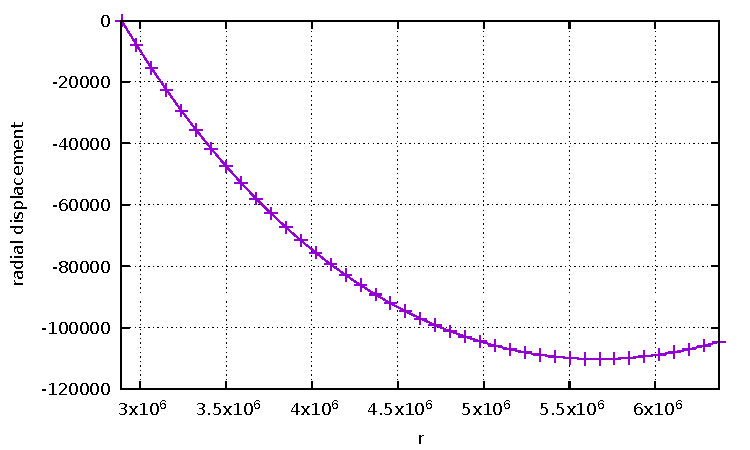
\includegraphics[width=7.5cm]{python_codes/fieldstone_36/displacement_rtheta.pdf}
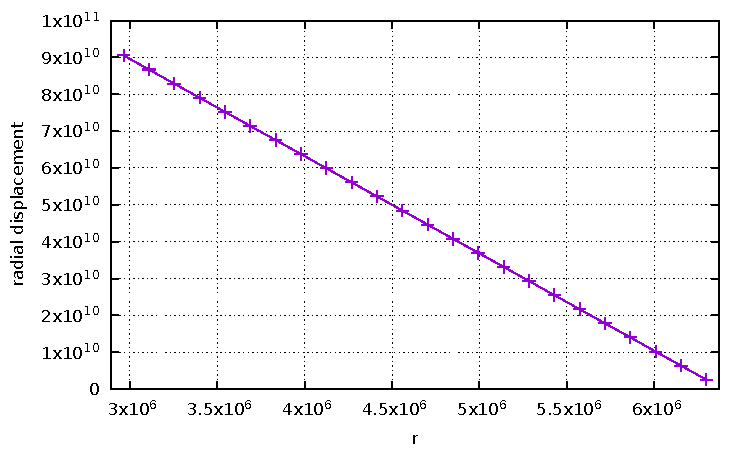
\includegraphics[width=7.5cm]{python_codes/fieldstone_36/pressure_rtheta.pdf}\\
{\small radial profiles of the displacement and pressure fields}
\end{center}

\begin{center}
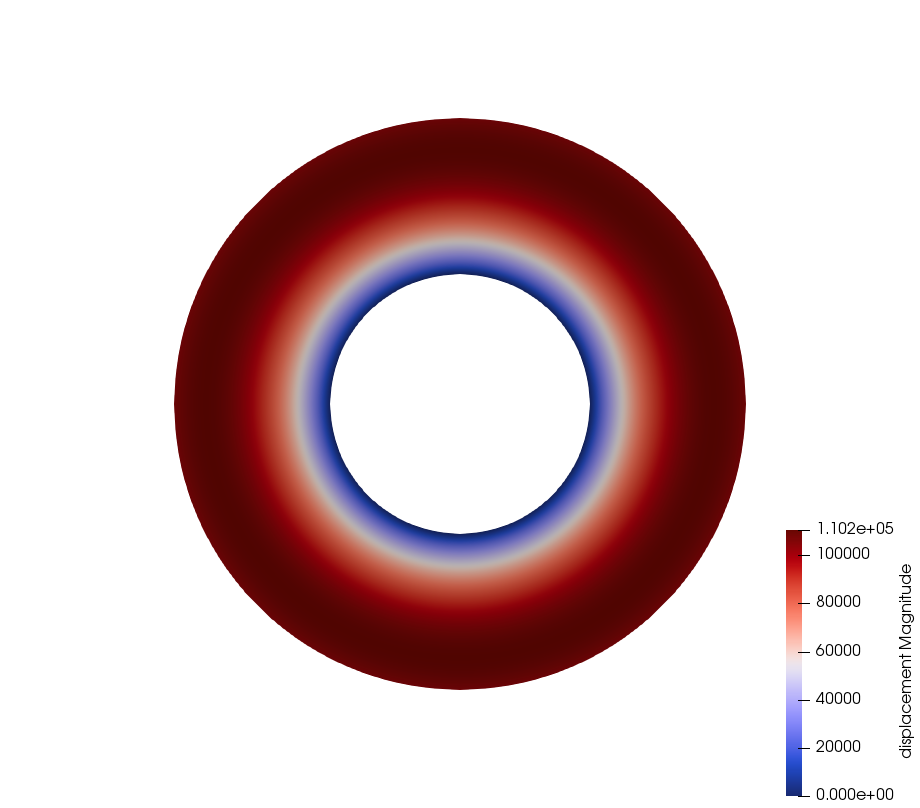
\includegraphics[width=7.5cm]{python_codes/fieldstone_36/disp}
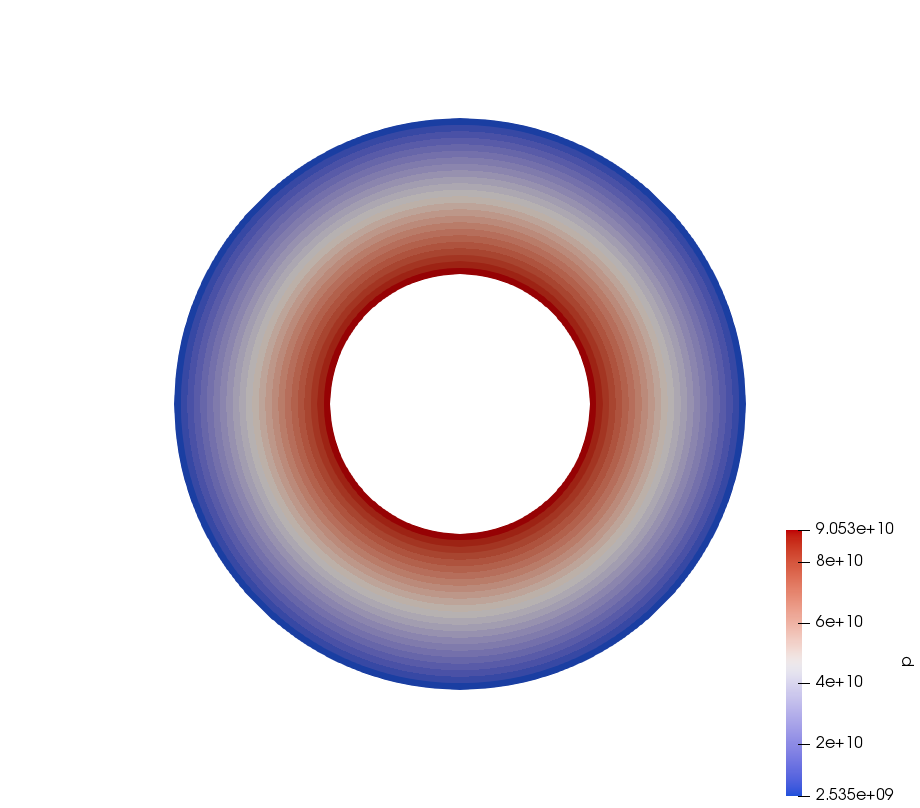
\includegraphics[width=7.5cm]{python_codes/fieldstone_36/p}\\
{\small displacement and pressure fields in the domain}
\end{center}

\begin{center}
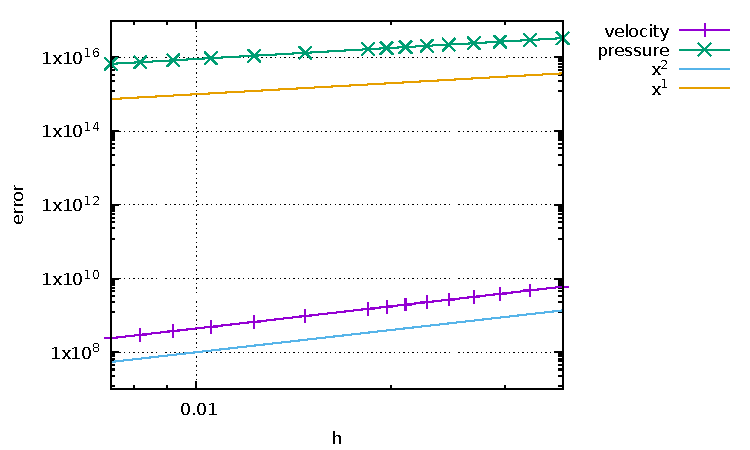
\includegraphics[width=16cm]{python_codes/fieldstone_36/errors}
\end{center}

